% document's head

\begin{center}
    \LARGE \textsc{Задание по курсу \\  <<Уравнения математической физики>>}
\end{center}

\hrule

\phantom{42}

\begin{flushright}
    \begin{tabular}{rr}
    % written by:
        % \textbf{Источник}: 
        % & \href{__ссылка__}{__название__} \\
        % & \\
        % \textbf{Лектор}: 
        % & _ФИО_ \\
        % & \\
        \textbf{Автор}: 
        & Хоружий Кирилл \\
        % & Примак Евгений \\
        & \\
    % date:
        \textbf{От}: &
        \textit{\today}\\
    \end{tabular}
\end{flushright}

\thispagestyle{empty}
% \tableofcontents
% \newpage




\subsection*{Теория}


Смещение длины волны при рассеянии (эффект Комптона):
\begin{equation}
    \Delta \lambda = \lambda_1 - \lambda_0 = \frac{h}{mc} \left(1 - \cos \theta\right).
\end{equation}
Считая, что $\varepsilon (\theta) = \frac{E_\gamma}{m c^2}= A N$ -- энергия рассеянных $\gamma$-квантов линейно зависит от номера соответствующего канала, найдём, что
\begin{equation}
    \frac{1}{N(\theta)} - \frac{1}{N(0)} = A (1 - \cos \theta),
    \hspace{10 mm} 
    m c^2 = E_\gamma(0) \frac{N_{90}}{N_0 - N_{90}},
\end{equation}
где $N_i$ -- номер канала, соотетствующего максимуму при угле в $i^{\circ}$, и $E_\gamma (0) = E_0$ -- энергия испускаемых источникм $\gamma$-квантов: $E_\gamma (0) = E_0 = 662$ кэВ.

\subsection*{Экспериментальная установка}

\textbf{Описание установки}. 1 -- блок питания; 2 -- тумблер включения питания образцов; 3 -- тумблер нагрева нити пирометра; 4 -- кнопка "Нагрев нити"; 5 -- кнопка "охлаждение нити"; 6
-- тумблер переключения образцов; 7 -- регулятор мощности нагрева образцов; 8 -- окуляр пирометра; 9 --
корпус пирометра; 10 -- объектив пирометра; 11 -- переключение диапазонов; 12 -- ручка смещения красного
светофильтра; 13 -- регулировочный винт; 14 -- вольтметр (напряжение на лампе накаливания); 15 -- амперметр (ток через образцы); 16 -- вольтметр в цепи термопары; 17 -- модель АЧТ; 18 трубка с кольцами из
материалов с различной излучательной способностью; 19 -- лампа накаливания; 20 -- неоновая лампочка.

\textbf{Описание образцов}. В работе исследуются:
\begin{itemize}
    \item \textit{Модель абсолютно чёрного тела} -- керамическая трубка, закрытая с одного конца и окружённая для теплоизоляции внешним кожухом. Температура в трубке измеряется с помощью термопары хромель-алюмель.
    \item \textit{Керамическая трубка с набором колец из различных материалов}, нагреваемая изнутри нихромовой спиралью. Материалы колец имеют различную излучательную способность.
    \item \textit{Вольфрамовая нить электрической лампочки}.
\end{itemize}

\begin{figure}[h]
    \centering
    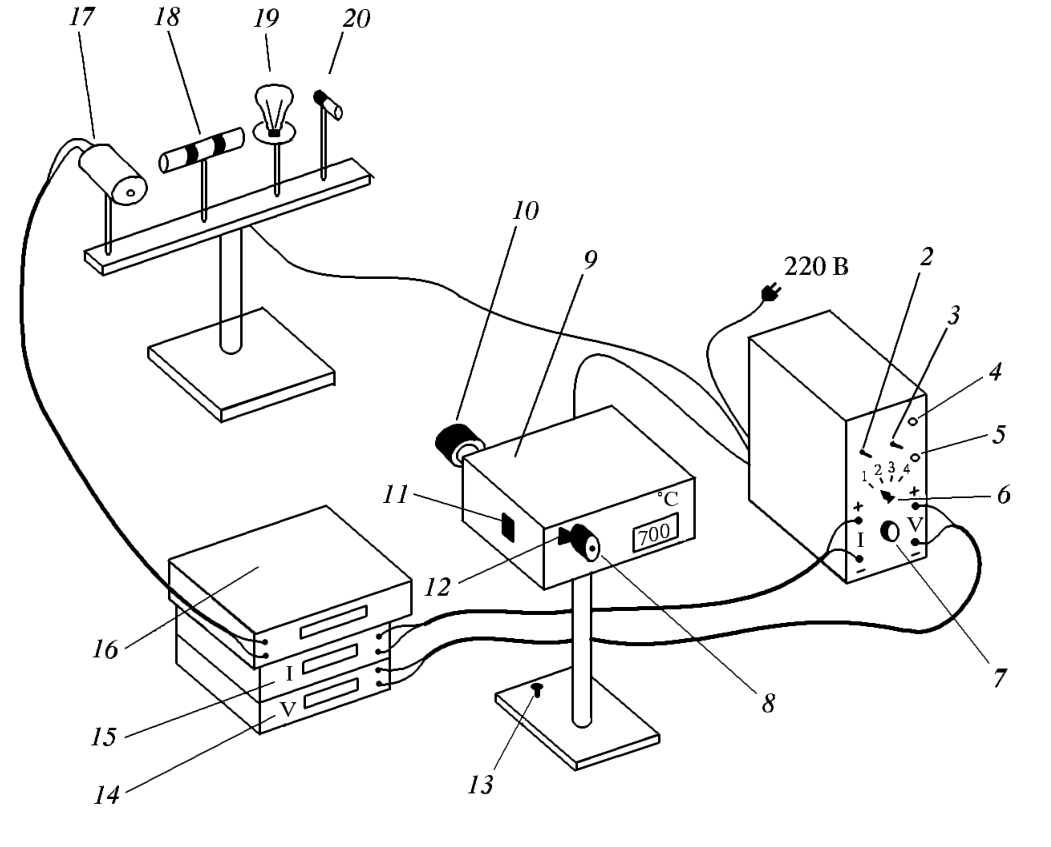
\includegraphics[width=0.6\textwidth]{imgs/exp.png}
    \caption{Схема экспериментальной установки}
    %\label{fig:}
\end{figure}


\newpage


\subsection*{Измерения}

\textbf{Изучение работы пирометра}. Нагрев АЧТ до красного каления (дождавшись стабилизации температуру, судя по показаниям термопары), с помощью пирометра измерим температуру $\sub{t}{pyr}$, сравним её с температурой, полученной по термопаре\footnote{
    Коэффициент перевода: $25.07 \cufrac{$\celc$}{мВ}$.
}  $\sub{t}{therm}$:
\begin{equation*}
    \sub{t}{therm} (45.89 \text{мВ})= 1150 \celc, 
    \hspace{5 mm} 
    \sub{t}{pyr} = [1137, 1140, 1144, 1155] \celc = [0.989, 0.991, 0.995, 1.004] \sub{t}{therm}.
\end{equation*}
Ошибка не превышает $2\%$, так что показанаиям пирометра, по крайней мере для АЧТ в этом диапазоне можно верить. 



\textbf{Изучение яркостной температуры накаленных тел}. Источником нагреваем керамическую трубку с кольцами из различных материалов. Пирометром измерели\footnote{
    Измерения проводлиоись несколько раз, что и обеспечило оценку погрешности каждого из измерений.
}  яркостную температуру поверхности трубки $\sub{t}{surf}$ и каждого из колец $\sub{t}{ring}^{(1)},\, \sub{t}{ring}^{(2)}$:
\begin{equation*}
    \sub{t}{surf} = (850 \pm 10) \celc,
    \hspace{5 mm} 
    \sub{t}{ring}^{(1)} \approx 794 \celc,
    \hspace{5 mm} 
    \sub{t}{ring}^{(2)} \approx 710 \celc.
\end{equation*}
Несовпадение яркостной тепературы обусловлено зависимостью мощности излучения от спектрального коэффициента поглощения, которой, видимо, различен для различных материалов второго образца.



\textbf{Проверка закона Стефана-Больцмана}. Теперь источником нагревается вольфрамовая нить лампы накаливания. С помощью пирометра измерялась яркостная температура нити $\sub{t}{thr}$ (в самом ярком месте). Параллельно снимались значения цифровыми мультиметрами снимались значения тока $I$ и напряжения $U$ на онной. Результаты можно найти в таблице №\ref{tab}.



\begin{table}[ht]
    \caption{Измерение яркостной температуры вольфрамовой нити, как функции мощности}
    \centering
    \begin{tabular}{rrrrrr}
    \toprule
       $U$, В &     $I$, А &    $N$, Вт &   $\Delta N$, Вт &    $t, \celc$ &  $\Delta t, \celc$ \\
    \midrule
    1.65 & 0.481 & 0.79 & 0.02 &  866 &  35 \\
    1.74 & 0.491 & 0.85 & 0.02 &  900 &  37 \\
    2.24 & 0.540 & 1.21 & 0.02 & 1000 &  40 \\
    2.57 & 0.572 & 1.47 & 0.03 & 1100 &  43 \\
    3.31 & 0.638 & 2.11 & 0.04 & 1200 &  46 \\
    3.29 & 0.635 & 2.09 & 0.04 & 1300 &  49 \\
    4.00 & 0.696 & 2.78 & 0.06 & 1400 &  52 \\
    4.74 & 0.754 & 3.57 & 0.07 & 1450 &  53 \\
    4.84 & 0.759 & 3.67 & 0.07 & 1500 &  55 \\
    4.59 & 0.742 & 3.41 & 0.07 & 1500 &  55 \\
    5.32 & 0.798 & 4.25 & 0.08 & 1600 &  58 \\
    6.13 & 0.857 & 5.25 & 0.11 & 1688 &  60 \\
    5.86 & 0.837 & 4.90 & 0.10 & 1700 &  61 \\
    7.00 & 0.915 & 6.40 & 0.13 & 1792 &  63 \\
    7.72 & 0.963 & 7.43 & 0.15 & 1800 &  64 \\
    7.51 & 0.949 & 7.13 & 0.14 & 1833 &  64 \\
    9.22 & 1.053 & 9.71 & 0.19 & 1900 &  67 \\
    \bottomrule
    \end{tabular}
\label{tab}
\end{table}


Погрешность измерения пирометра на основе предыдующих измерений была положена $\sim 3\% \pm 10$, для мультиметров взят $\sim 1\%$ от показаний.


\textbf{Измерение яркостной температуры неоновой лампочки}. Включив неоновую лампочку, пирометром измерим её яркостную температуру $\sub{t}{Ne}$:
\begin{equation*}
    \sub{t}{Ne} = (874 \pm 27) \celc,
\end{equation*}
что, очевидно $\gg 30 \celc$. Ну, так совпало, что переход электронов между энергетическими уровнями неона имеет длину волны схожую, с излучением АЧТ на измеренной температуре. 
\newpage
\subsection*{Обработка данных}


В логарифмическом масштабе построим $\ln(U \times  I)[\ln(\sub{t}{surf})]$. Начиная с температуры $\sub{t}{surf} \sim 1500 \celc$ (красная точка на графике) вольфрамовая нить светилась почти полностью, начиная с этой температуры приближаем из соображений
\begin{equation*}
    UI = W = \varepsilon_T B T^n, 
    \hspace{0.5cm} \Rightarrow \hspace{0.5cm}
    \ln W = \ln(\varepsilon_T B) + n \ln (T).
\end{equation*}
Лабораторный практикум предлагает игнорировать зависимость $\varepsilon_T (\sub{t}{surf})$, однако это вносит достаточно существенные изменения, поэтому данные из таблицы лабораторного пракикума (таблица №1, стр. 236) восттановили зависимость $\varepsilon_T (T)$.  
\vspace{-5mm}

\begin{figure}[h]
    \centering
    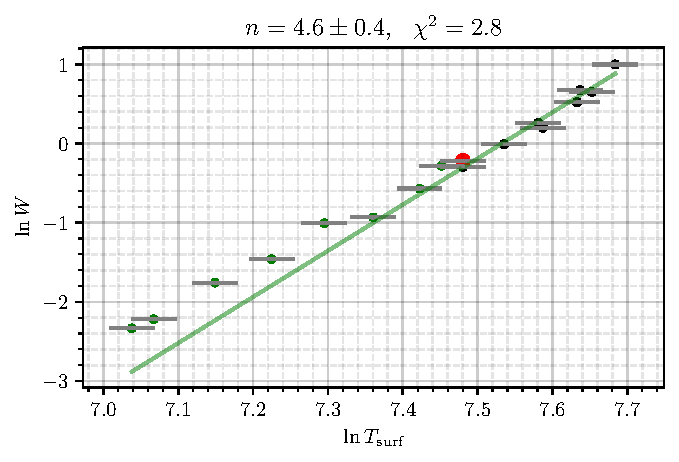
\includegraphics[width=0.6\textwidth]{figs/fig2.pdf}
    \vspace{-5mm}
    \caption{Приближение зависимости $W(\sub{t}{surf})$}
    \label{fig:plot}
\end{figure}


Значения $\chi^2 = 2.8$ говорит об адекватности приближения в рамках данной погрешности. 
Итого, находим значение для $n$
\begin{equation*}
    n = 4.8 \pm 0.4,
\end{equation*}
что, учетом погрешности, сходится с ожиданиями. 

Теперь определим постоянную Стефана-Бльцмана. Основной вклад в погрешность даёт температура в силу $T^4$. Также наблюдается постоянный сдвиг, скорее всего связанный с неточностью указанной $S = 0.36 \text{ см}^2$, измерить которую не представляется возможным (значение лучше сходится с табличным при $S = 0.27 \text{ см}^2$). 

\begin{figure}[h]
    \centering
    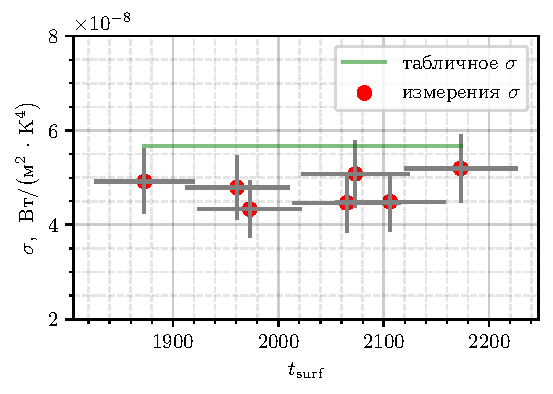
\includegraphics[width=0.5\textwidth]{figs/fig3.pdf}
    \vspace{-5mm}
    \caption{Сравнение полученных значений постоянной Стефана-Больцмана с табличным значением}
    %\label{fig:}
\end{figure}

\subsection*{Выводы}

Исследована зависимость пропускающей способности от толщины образца для свинца, железа, алюминия и пробки. Можно заметитьЮ что чем плотнее вещество, тем выше коэффциент ослабления. Измерены коэффциенты ослабления для указанных веществ.

 По значениям коэффциента ослабления, получено значение энергии $\gamma$-квантов: $E \approx 0.8$ МэВ. В пределах погрешности значения энергии для трёх веществ совпали. 






 \subsection*{Счётчик Гейгера}


 Также, параллельно с вышеописанной работой было произведено знакомство с прибором для измерения радиационного фона. 

 На рабочем месте уровень радиации составил 15 мкР/час. Вблизи пучка счётчик начинает зашкаливать на значениях более 999 мкР/час. Отдаляясь на 5 см от пучка, наблюдалось значение в районе 60 мкР/час, и на расстояние в районе 10 см, уже 26 мкр/час -- пучок действительно коллимированный.


% К тому же $\vc{\tilde{\bar{\alpha}}} + \sqrt{\alpha} + \beta$ просто так.
% \begin{equation*}
%     \begin{pmatrix}
%         1 & 2  \\
%         3 & 3  \\
%     \end{pmatrix}
% \end{equation*}
% Хочется, чтобы
% \begin{equation*}
%     \begin{pmatrix}
%         1 & 2 & 3 \\
%         35 & 5 & 5 \\
%         5 & 5 & 66 \\
%     \end{pmatrix}
% \end{equation*}
% Lorem ipsum dolor sit amet, consectetur adipisicing elit, sed do eiusmod
% tempor incididunt ut labore et dolore magna aliqua. Ut enim ad minim veniam,
% quis nostrud exercitation ullamco laboris nisi ut aliquip ex ea commodo
% consequat. Duis aute irure dolor in reprehenderit in voluptate velit esse
% cillum dolore eu fugiat nulla pariatur. Excepteur sint occaecat cupidatat non
% proident, sunt in culpa qui officia deserunt mollit anim id est laborum.
% \begin{equation*}
%     c_1{}^5 \cos ^5(k t)+c_2{}^5 \sin ^5(k t)+10 c_1{}^3 c_2{}^2 \sin ^2(k t) \cos ^3(k t)+10 c_1{}^2 c_2{}^3 \sin ^3(k t) \cos ^2(k t)+5 c_1{}^4 c_2 \sin (k t) \cos ^4(k t)+5 c_1 c_2{}^4 \sin ^4(k t) \cos (k t)
% \end{equation*}